\documentclass{standalone}
\usepackage{tikz, pgf}
\usetikzlibrary{arrows, automata, backgrounds, positioning, shapes}
\pagestyle{empty}

\begin{document}
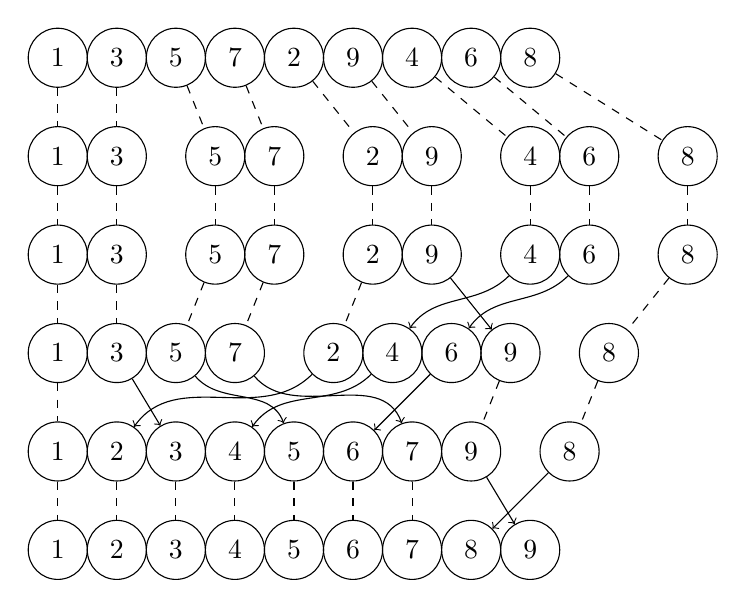
\begin{tikzpicture}

\tikzstyle{every node}=[draw,shape=circle,minimum width=0.75cm,minimum height=0.75cm,anchor=center];

\node (r01) at (1*0.75,0){1};
\node (r02) at (2*0.75,0){3};
\node (r03) at (3*0.75,0){5};
\node (r04) at (4*0.75,0){7};
\node (r05) at (5*0.75,0){2};
\node (r06) at (6*0.75,0){9};
\node (r07) at (7*0.75,0){4};
\node (r08) at (8*0.75,0){6};
\node (r09) at (9*0.75,0){8};

\node (r11) at (1*0.75,-1.25){1};
\node (r12) at (2*0.75,-1.25){3};
\node (r13) at (3*0.75+0.5,-1.25){5};
\node (r14) at (4*0.75+0.5,-1.25){7};
\node (r15) at (5*0.75+1,-1.25){2};
\node (r16) at (6*0.75+1,-1.25){9};
\node (r17) at (7*0.75+1.5,-1.25){4};
\node (r18) at (8*0.75+1.5,-1.25){6};
\node (r19) at (9*0.75+2,-1.25){8};

\node (r21) at (1*0.75,-2.5){1};
\node (r22) at (2*0.75,-2.5){3};
\node (r23) at (3*0.75+0.5,-2.5){5};
\node (r24) at (4*0.75+0.5,-2.5){7};
\node (r25) at (5*0.75+1,-2.5){2};
\node (r26) at (6*0.75+1,-2.5){9};
\node (r27) at (7*0.75+1.5,-2.5){4};
\node (r28) at (8*0.75+1.5,-2.5){6};
\node (r29) at (9*0.75+2,-2.5){8};

\node (r31) at (1*0.75,-3.75){1};
\node (r32) at (2*0.75,-3.75){3};
\node (r33) at (3*0.75,-3.75){5};
\node (r34) at (4*0.75,-3.75){7};
\node (r35) at (5*0.75+0.5,-3.75){2};
\node (r36) at (6*0.75+0.5,-3.75){4};
\node (r37) at (7*0.75+0.5,-3.75){6};
\node (r38) at (8*0.75+0.5,-3.75){9};
\node (r39) at (9*0.75+1,-3.75){8};

\node (r41) at (1*0.75,-5){1};
\node (r42) at (2*0.75,-5){2};
\node (r43) at (3*0.75,-5){3};
\node (r44) at (4*0.75,-5){4};
\node (r45) at (5*0.75,-5){5};
\node (r46) at (6*0.75,-5){6};
\node (r47) at (7*0.75,-5){7};
\node (r48) at (8*0.75,-5){9};
\node (r49) at (9*0.75+0.5,-5){8};

\node (r51) at (1*0.75,-6.25){1};
\node (r52) at (2*0.75,-6.25){2};
\node (r53) at (3*0.75,-6.25){3};
\node (r54) at (4*0.75,-6.25){4};
\node (r55) at (5*0.75,-6.25){5};
\node (r56) at (6*0.75,-6.25){6};
\node (r57) at (7*0.75,-6.25){7};
\node (r58) at (8*0.75,-6.25){8};
\node (r59) at (9*0.75,-6.25){9};

\draw (r01) edge[dashed] (r11)
(r02) edge[dashed] (r12)
(r03) edge[dashed] (r13)
(r04) edge[dashed] (r14)
(r05) edge[dashed] (r15)
(r06) edge[dashed] (r16)
(r07) edge[dashed] (r17)
(r08) edge[dashed] (r18)
(r09) edge[dashed] (r19);

\draw (r11) edge[dashed] (r21)
(r12) edge[dashed] (r22)
(r13) edge[dashed] (r23)
(r14) edge[dashed] (r24)
(r15) edge[dashed] (r25)
(r16) edge[dashed] (r26)
(r17) edge[dashed] (r27)
(r18) edge[dashed] (r28)
(r19) edge[dashed] (r29);

\draw (r21) edge[dashed] (r31)
(r22) edge[dashed] (r32)
(r23) edge[dashed] (r33)
(r24) edge[dashed] (r34)
(r25) edge[dashed] (r35)
(r26) edge[->] (r38)
(r27) edge[->,out=225,in=55] (r36)
(r28) edge[->,out=225,in=55] (r37)
(r29) edge[dashed] (r39);

\draw (r31) edge[dashed] (r41)
(r32) edge[->] (r43)
(r33) edge[->,out=310,in=110] (r45)
(r34) edge[->,out=310,in=110] (r47)
(r35) edge[->,out=225,in=55] (r42)
(r36) edge[->,out=225,in=55] (r44)
(r37) edge[->] (r46)
(r38) edge[dashed] (r48)
(r39) edge[dashed] (r49);

\draw (r41) edge[dashed] (r51)
(r42) edge[dashed] (r52)
(r43) edge[dashed] (r53)
(r44) edge[dashed] (r54)
(r45) edge[dashed] (r55)
(r46) edge[dashed] (r56)
(r47) edge[dashed] (r57)
(r48) edge[->] (r59)
(r49) edge[->] (r58);

\end{tikzpicture}
\end{document}
